\documentclass{ctexart}
\usepackage{geometry}
\usepackage{diagbox}
\usepackage{graphicx}
\usepackage{subfigure}
\usepackage{amsmath}
\usepackage{amssymb}
\usepackage{indentfirst}
\usepackage{xfrac}
\usepackage{color}
\usepackage[table]{xcolor}
\usepackage{multirow}
\usepackage{titlesec}
\usepackage{bm}
\usepackage{caption}
\title{基于LSTM的风力系统上网功率预测}
\author{未央-能动02\quad 徐智昱\quad 2020012991}
\date{}
\begin{document}
\maketitle
\begin{abstract}
    在双碳目标下,根据历史数据对风电机未来一段时间内的运行状况结合其它设施进行调峰具有重大意义。本研究采用实际获得的风电机组一个月的运行数据
    与当地一个月的风力数据,进行未来1小时每15分钟一个点的功率预测。风电机的功率与当地风速有着紧密关系,而风速与风功率也有明显的自回归现象,
    因此考虑能够考虑这种自回归与相关性的模型进行建模。循环神经网络(RNN)就是这样一种方法,本研究采用了长短期记忆网络(LSTM)对风功率的预测进行了研究,
    并通过调整参数试图找到较为适合的模型。同时,也考虑利用传统的时间序列分析(TSA)的方法对此数据进行考量,比较经典方法与现代方法之间效果的差异。
\end{abstract}
\textbf{关键词:} TSA, RNN, LSTM
\section{引言}
\subsection{数据描述与预处理}
获得的风电数据来自江苏的风电场,包含风速与风功率两组变量,在2015/10/1 0:00到2015/10/31 23:59被采集,每30秒采集一次数据,
内有一系列缺失数据。根据国家标准,需要对未来1个小时的4个,每个间隔15分钟的点进行预测,因此将数据集每15个点进行合并,可以借此作出散点图
与时序图。\\
\begin{figure}[htbp]
    \centering
    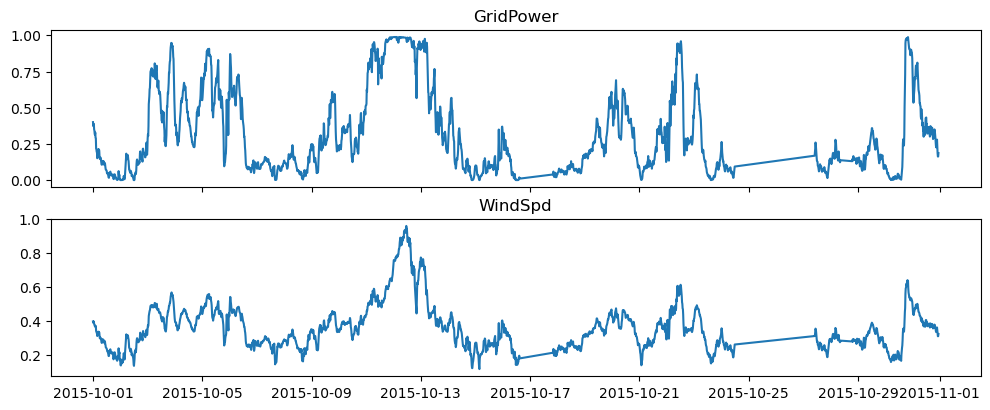
\includegraphics[width=0.80\textwidth]{photos/original_time_series.png}
    \caption{原始数据时序图}
\end{figure}
由时序图可以发现其存在较多的时间缺失区间,因此在实际建立模型时选择使用分段的区间进行模型的训练,放弃具有缺失值的部分。\\
\indent 同时可以作出的风功率与风速关系的图像,并同时用Kernel Regression对数据符合的形式作初步的拟合,结果如下图所示:\\
\begin{figure}[htbp]
    \centering
    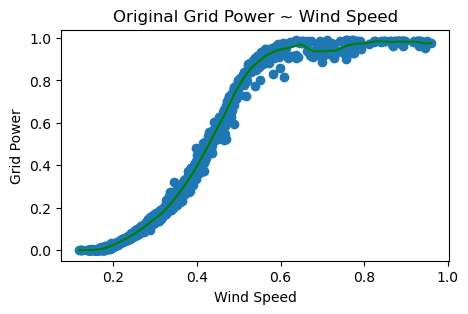
\includegraphics[width = 0.6\textwidth]{photos/scatter_fitted.png}
    \caption{风功率风速关系图}
\end{figure}
由图可见,二者关系可能近似符合类似于Logistic Function的形式;同时可能经过恰当的变换后,可以找到用于描述的线性函数描述其变化。\\
\indent 在时间序列中,常用的检测离群值(Outlier)的方法是认为每个数据独立同分布地服从于正态分布,由正态分布的置信区间判断有无明显的离群值。
利用这个方法可以作出此数据的离群值:\\
\begin{figure}[htbp]
    \centering
    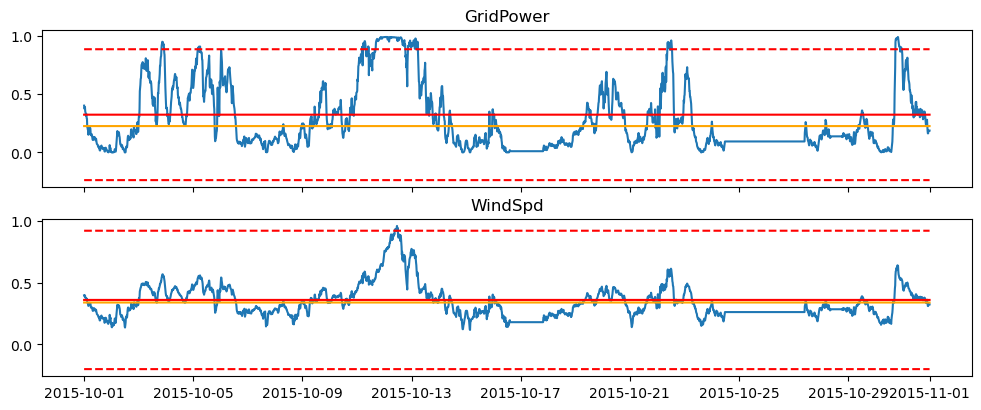
\includegraphics[width=0.80\textwidth]{photos/outliers.png}
    \caption{离群值检测}
\end{figure}
由图像可以发现,数据的特性良好,存在极少的离群值,因此不需要对数据的离群值进行处理。\\
\indent 由图1可见,数据实际上存在较多的噪音,因此考虑使用滑动平均(Moving Average)的方法,降低数据的噪音。下图是以20个数据点为窗口的滑动平均的结果:\\
\begin{figure}[htbp]
    \centering
    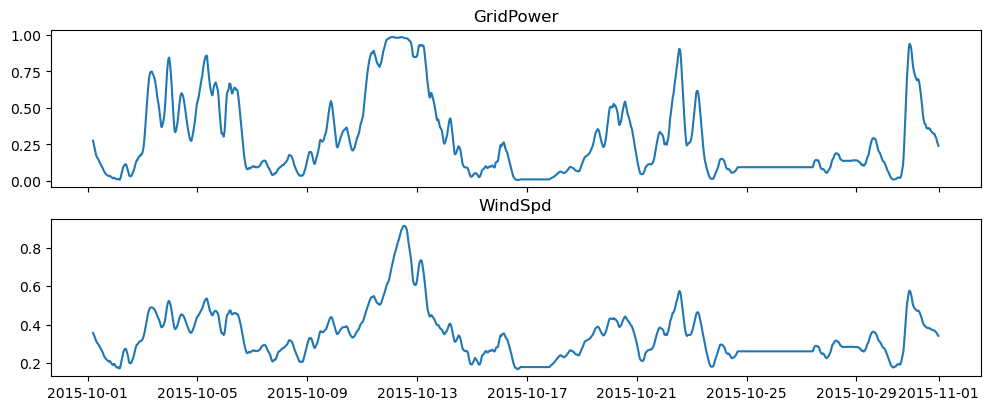
\includegraphics[width = 0.8\textwidth]{photos/ma_time_series.png}
    \caption{滑动平均数据}
\end{figure}
滑动平均后数据明显变得光滑,但也失去了一部分的信息,将对滑动平均前后分别建立模型进行研究来探究实际中应该使用何种模型进行
训练。\\
\end{document}